\documentclass[twocolumn]{article}
\usepackage{graphicx}
\usepackage{amsmath, amssymb, amsfonts}
\usepackage{geometry}
\usepackage{tikz}
\usetikzlibrary{arrows.meta, positioning, shapes.geometric, calc}
\usepackage{caption}
\usepackage{hyperref}
\usepackage{booktabs}
\usepackage{multirow}

\geometry{a4paper, left=20mm, right=20mm, top=25mm, bottom=25mm}

\title{\textbf{Draft Report: Integrating Brain-Computer Interfaces with Adaptive AI}}
\author{Student ID: 11314389}
\date{\today}

\begin{document}

\maketitle

\section{Introduction}

Research in motor imagery Brain--Computer Interfaces (BCIs) has delivered impressive offline classification accuracies, yet two structural barriers block real-world deployment. First, electroencephalogram (EEG) signals are notoriously non-stationary. Any static decoder---whether handcrafted CSP+LDA or deep convolutional networks---tends to overfit the calibration session; as soon as the neural state drifts, accuracy collapses. Second, even when classification works, the pipeline remains open-loop: the predicted label is mapped directly to a rigid command, making it difficult to generate smooth, corrective actions for robotic end-effectors.

Classical pipelines rely on OVR-CSP to maximise class variance ratios, followed by linear classifiers that assume a stationary feature manifold. Deep neural nets improve representation learning but still operate as one-shot recognisers, lacking the feedback needed to adapt to drift or to arbitrate between task goals and noisy sensory evidence. As a result, conventional decoders struggle to produce continuous, stable trajectories suitable for robot control.

This project explores a new hypothesis: by reframing BCI decoding as a sequential decision-making problem, we can leverage reinforcement learning (RL) to close the loop. Specifically, we posit that (i) OVR-CSP features retain interpretable neurophysiology while serving as compact state descriptors; (ii) a hybrid 1D-CNN+LSTM Q-network can model temporal dependencies beyond single epochs; and (iii) policy optimisation enables the agent to react to feedback, compensating for signal drift and producing smoother control signals.

To validate generalisation, we evaluate the pipeline on two complementary BCI Competition IV datasets: IV-2a (22-channel, 4-class) and IV-2b (3-channel, 2-class, multi-session). This dual-dataset strategy tests robustness across electrode montages, class counts, and inter-session variability. Figure~\ref{fig:system_overview} sketches the resulting pipeline.

\section{Methodology}

This chapter documents the end-to-end system devised to translate raw EEG into robotic control commands. The current implementation contains three fully operational phases---data processing, feature engineering, and reinforcement-learning training---plus a planned execution phase for simulation and robot deployment.

\subsection{Phase 1: Data Acquisition \& Preprocessing}

\subsubsection{Dataset Selection and Comparative Rationale}
This project employs two complementary datasets from the BCI Competition IV suite to validate generalisation and robustness:

\textbf{Dataset IV-2a} comprises 22-channel EEG from 9 subjects performing four-class motor imagery (left hand, right hand, feet, tongue). It serves as the primary benchmark due to its widespread adoption in MI-BCI literature, enabling direct comparison with state-of-the-art methods.

\textbf{Dataset IV-2b} provides 3-channel EEG (C3, Cz, C4) from 9 subjects performing binary left/right hand imagery across five sessions. Its reduced channel count and multi-session structure allow us to (i) evaluate robustness under limited spatial resolution, and (ii) assess cross-session generalisation---a critical requirement for practical deployment.

By training and evaluating on both datasets, we test whether the proposed pipeline generalises across different electrode montages, class counts, and inter-session variability, rather than overfitting to a single experimental paradigm.

\subsubsection{Neurophysiological Basis}
Motor imagery (MI) elicits event-related desynchronisation/synchronisation (ERD/ERS) in the Mu (8--13\,Hz) and Beta (13--30\,Hz) bands over the contralateral sensorimotor cortex \cite{hameed2025enhancing}. These modulations provide the electrophysiological signatures exploited downstream.

\subsubsection{Spectral Filtering Strategy}
MNE-Python implements a zero-phase FIR bandpass to retain the informative band:
\begin{align}
    x_{\text{band}}(t) &= \mathcal{F}^{-1}\{H(\omega)\mathcal{F}[x(t)]\}, \\
    H(\omega) &=
    \begin{cases}
        1, & \omega\in[8,30]\text{ Hz},\\
        0, & \text{otherwise.}
    \end{cases}
\end{align}
The passband suppresses EOG-dominated low frequencies and EMG-rich high frequencies while retaining ERD/ERS dynamics.

\subsubsection{Artifact Removal via ICA}
Independent component analysis isolates ocular artefacts:
\begin{equation}
    X = AS,\qquad \hat{S}=WX.
\end{equation}
Components strongly correlated with dedicated EOG channels form the rejection set $\mathcal{I}_{\text{bad}}$, yielding cleaned signals
\begin{equation}
    \tilde{X}=A\tilde{S},\qquad \tilde{S}_{i}=0\ \text{if}\ i\in\mathcal{I}_{\text{bad}}.
\end{equation}

\subsubsection{Epoching and Output Artifacts}
Cue-locked windowing produces tensors $X\in\mathbb{R}^{N\times C\times T}$. Each subject’s cleaned raw, ICA report, and epoch data are persisted in \texttt{.fif} format. Amplitudes remain on the physical scale; optional normalisation is reserved for future experiments.

\begin{figure*}[t]
    \centering
\resizebox{0.95\textwidth}{!}{%
    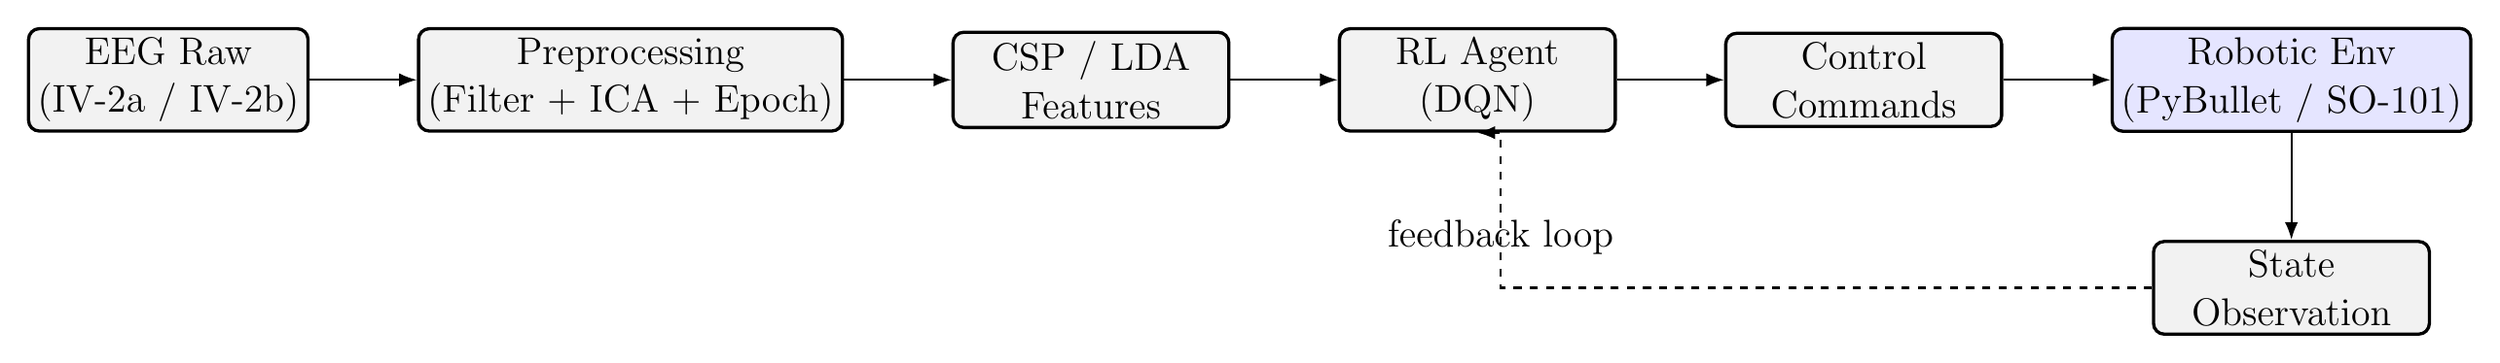
\begin{tikzpicture}[
      node distance=11mm and 14mm,
      block/.style={rectangle, rounded corners, draw, very thick,
                    minimum width=36mm, minimum height=12mm,
                    align=center, fill=gray!10, font=\Large},
      envblock/.style={rectangle, rounded corners, draw, very thick,
                    minimum width=36mm, minimum height=12mm,
                    align=center, fill=blue!10, font=\Large},
      arrow/.style={-Latex, thick},
      every node/.style={font=\Large}
    ]
        \node[block] (raw) {EEG Raw\\(IV-2a / IV-2b)};
        \node[block, right=of raw] (prep) {Preprocessing\\(Filter + ICA + Epoch)};
        \node[block, right=of prep] (csp) {CSP / LDA\\Features};
        \node[block, right=of csp] (dqn) {RL Agent\\(DQN)};
        \node[block, right=of dqn] (ctrl) {Control\\Commands};
        \node[envblock, right=of ctrl] (robot) {Robotic Env\\(PyBullet / SO-101)};
        \node[block, below=of robot, yshift=-3mm] (obs) {State\\Observation};
        \draw[arrow] (raw) -- (prep);
        \draw[arrow] (prep) -- (csp);
        \draw[arrow] (csp) -- (dqn);
        \draw[arrow] (dqn) -- (ctrl);
        \draw[arrow] (ctrl) -- (robot);
        \draw[arrow] (robot) -- (obs);
        \draw[arrow, dashed] (obs.west) -- ++(-85mm,0) |- (dqn.south) node[pos=0.25, below]{\Large feedback loop};
    \end{tikzpicture}}
    \caption{End-to-end preprocessing-to-control flow. The RL agent receives CSP features from EEG, outputs discrete commands to the robotic environment (simulated or physical), and receives state observations forming a closed-loop control system.}
    \label{fig:pipeline_flow}
\end{figure*}

\begin{figure*}[t]
    \centering
\resizebox{\textwidth}{!}{%
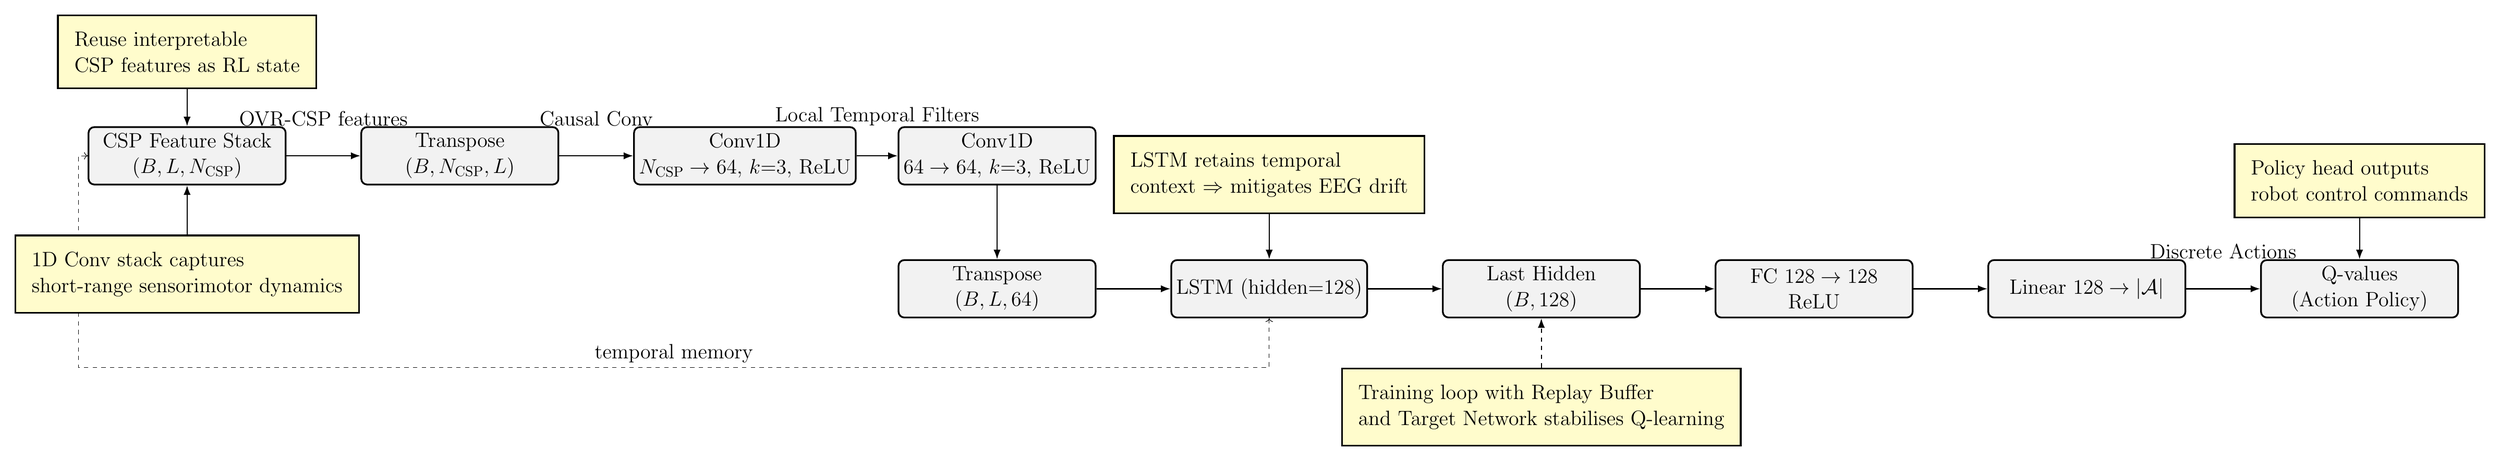
\begin{tikzpicture}[
      node distance=15mm and 18mm,
      block/.style={rectangle, rounded corners, draw, very thick, fill=gray!10,
                    minimum width=48mm, minimum height=14mm, align=center, font=\Large},
      annot/.style={rectangle, draw, very thick, fill=yellow!20,
                    inner sep=4mm, font=\Large, align=left},
      arrow/.style={-Latex, thick},
      every node/.style={font=\Large}
    ]
    \node[block] (input) {CSP Feature Stack\\$(B,L,N_{\text{CSP}})$};
    \node[block, right=of input] (transpose1) {Transpose\\$(B,N_{\text{CSP}},L)$};
    \node[block, right=of transpose1] (conv1) {Conv1D\\$N_{\text{CSP}}\rightarrow64$, $k{=}3$, ReLU};
    \node[block, right=of conv1, xshift=-8mm] (conv2) {Conv1D\\$64\rightarrow64$, $k{=}3$, ReLU};
    \node[block, below=of conv2, yshift=-3mm] (transpose2) {Transpose\\$(B,L,64)$};
    \node[block, right=of transpose2, minimum width=40mm] (lstm) {LSTM (hidden=128)};
    \node[block, right=of lstm] (select) {Last Hidden\\$(B,128)$};
    \node[block, right=of select] (fc1) {FC $128\rightarrow128$\\ReLU};
    \node[block, right=of fc1] (fc2) {Linear $128\rightarrow|\mathcal{A}|$};
    \node[block, right=of fc2] (output) {Q-values\\(Action Policy)};

    \draw[arrow] (input) -- node[above=6mm]{\Large OVR-CSP features} (transpose1);
    \draw[arrow] (transpose1) -- node[above=6mm]{\Large Causal Conv} (conv1);
    \draw[arrow] (conv1) -- node[above=6mm]{\Large Local Temporal Filters} (conv2);
    \draw[arrow] (conv2) -- (transpose2);
    \draw[arrow] (transpose2) -- (lstm);
    \draw[arrow] (lstm) -- (select);
    \draw[arrow] (select) -- (fc1);
    \draw[arrow] (fc1) -- (fc2);
    \draw[arrow] (fc2) -- node[above=6mm]{\Large Discrete Actions} (output);

    \coordinate (tmA) at ($(lstm.south)+(0,-12mm)$);
    \coordinate (tmB) at ($(tmA)+(-290mm,0)$);
    \coordinate (tmC) at (tmB |- input.west);
    \draw[<->, dashed] (lstm.south) -- (tmA) -- (tmB)
        node[above, pos=0.5]{\Large temporal memory}
        -- (tmC) -- (input.west);

    \node[annot, above=9mm of input] (anno1) {Reuse interpretable\\CSP features as RL state};
    \node[annot, below=12mm of input] (anno2) {1D Conv stack captures\\short-range sensorimotor dynamics};
    \node[annot, above=11mm of lstm] (anno3) {LSTM retains temporal\\context $\Rightarrow$ mitigates EEG drift};
    \node[annot, above=10mm of output] (anno4) {Policy head outputs\\robot control commands};
    \node[annot, below=12mm of select, minimum width=56mm] (anno5) {Training loop with Replay Buffer\\and Target Network stabilises Q-learning};

    \draw[arrow] (anno1.south) -- (input.north);
    \draw[arrow] (anno2.north) -- (input.south);
    \draw[arrow] (anno3.south) -- (lstm.north);
    \draw[arrow] (anno4.south) -- (output.north);
    \draw[arrow, dashed] (anno5.north) -- (select.south);
    \end{tikzpicture}}
    \caption{Overview of the proposed BCI control pipeline.}
    \label{fig:system_overview}
\end{figure*}

\subsection{Phase 2: Feature Engineering \& Baseline}

\subsubsection{One-vs-Rest CSP}
For each class $k$, common spatial patterns solve
\begin{equation}
    \Sigma_k w=\lambda(\Sigma_k+\Sigma_{\neg k})w,\qquad
    J(w) = \frac{w^\top \Sigma_k w}{w^\top \Sigma_{\neg k} w},
\end{equation}
producing filters $W$ and log-variance features $f_i$. The inverse matrix $P = W^{-1}$ supports topographic verification.

\subsubsection{Baseline Classifier and Evaluation Protocol}
CSP features feed an LDA classifier evaluated via stratified 5-fold cross-validation. For each fold, 80\% of trials are used for training and 20\% for testing, with stratification ensuring class balance across splits. We report per-subject accuracy, macro-averaged precision/recall, and aggregate confusion matrices.

Additionally, a deep learning baseline using the CTNet architecture \cite{prev_student2024} is trained under identical data splits. This two-tier baseline (classical CSP+LDA vs.\ deep CTNet) establishes performance bounds against which the RL agent is compared.

The resulting metrics, filters, and transformed features are exported (\texttt{csp\_features.npz}, \texttt{csp\_filters.npy}, \texttt{csp\_patterns.npy}, \texttt{csp\_metrics.json}), ensuring the RL module consumes identical representations.

\subsection{Phase 3: RL Framework Definition}

We reformulate control as an MDP \cite{nallani2024rleegnet}; Table~\ref{tab:mdp_spec} summarises the specification.

\begin{table}[t]
    \centering
    \caption{\textbf{Specification of the MDP used for BCI control.}}
    \label{tab:mdp_spec}
    \renewcommand{\arraystretch}{1.18}
    \begin{tabular}{@{}p{0.26\columnwidth} p{0.68\columnwidth}@{}}
        \toprule
        Component & Definition / Description \\
        \midrule
        State $s_t$ & Stack of the latest $L$ CSP feature vectors ($s_t \in \mathbb{R}^{L\times N_{\text{CSP}}}$), aligned with the replay buffer tensors. \\
        Action $a_t$ & Discrete end-effector commands $\{\text{Left, Right, Up, Down}\}$. \\
        Reward $r_t$ & Label-aligned signal $r_t \in \{+1,-\lambda\}$ used for current offline training; environment rewards will replace this during closed-loop deployment. \\
        Transition $\mathcal{P}$ & Offline updates sample $(s_{t+1})$ from stored transitions; simulators/hardware will provide $s_{t+1}\sim\mathcal{P}(\cdot|s_t,a_t)$. \\
        Discount $\gamma$ & Default $\gamma = 0.99$ balances short- and long-term objectives. \\
        \bottomrule
    \end{tabular}
\end{table}

\subsubsection{Function Approximation}
The Q-function $Q(s,a;\theta)$ is implemented using the network detailed in Table~\ref{tab:net_arch}.

% \begin{figure}[t]
%     \centering
%     \fbox{\begin{minipage}{0.95\columnwidth}
%         \centering
%         \vspace{1.0cm}\textbf{[Insert Compact Network Diagram Here]}\\
%         \textit{1D-CNN + LSTM Q-network.}
%         \vspace{1.0cm}
%     \end{minipage}}
%     \caption{Column-width illustration of the policy network.}
%     \label{fig:network}
% \end{figure}

\begin{table}[t]
    \centering
    \caption{\textbf{Architecture details of the 1D-CNN+LSTM Q-network.}}
    \label{tab:net_arch}
    \setlength{\tabcolsep}{5pt}
    \renewcommand{\arraystretch}{1.12}
    \begin{tabular}{@{}p{0.22\columnwidth} p{0.48\columnwidth} p{0.25\columnwidth}@{}}
        \toprule
        Layer & Parameters & Output Shape \\
        \midrule
        Input & CSP feature stack & $(B, L, N_{\text{CSP}})$ \\
        Conv1 & $N_{\text{CSP}}\!\rightarrow\!64$, $k=3$, $p=1$, ReLU & $(B, L, 64)$ \\
        Conv2 & $64\!\rightarrow\!64$, $k=3$, $p=1$, ReLU & $(B, L, 64)$ \\
        LSTM & hidden=128, layers=1 & $(B, L, 128)$ \\
        FC & $128\rightarrow128$, ReLU & $(B, 128)$ \\
        Output & $128\rightarrow|\mathcal{A}|$, Linear & $(B, 4)$ \\
        \bottomrule
    \end{tabular}
\end{table}

\subsubsection{Training Mechanism}
Experience replay, a softly updated target network, and Huber loss
\begin{equation}
    L_\delta(y,Q) =
    \begin{cases}
        \tfrac{1}{2}(y-Q)^2, & |y-Q| \le \delta \\
        \delta(|y-Q| - \tfrac{1}{2}\delta), & \text{otherwise}
    \end{cases}
\end{equation}
stabilise training, with $y = r_t + \gamma \max_{a'} Q_{\text{target}}(s_{t+1},a';\theta^-)$.

\subsubsection{RL Evaluation Protocol}
To prevent overfitting and ensure fair comparison, the RL agent follows a trial-based data split:
\begin{itemize}
    \item \textbf{Training set (80\%)}: Trials are randomly sampled with stratification by class label. The $\varepsilon$-greedy exploration policy ($\varepsilon$ decaying from 1.0 to 0.01) guides action selection during training.
    \item \textbf{Test set (20\%)}: Held-out trials never seen during training. During evaluation, the exploration policy is disabled (pure exploitation, $\varepsilon=0$), and the greedy action $a^* = \arg\max_a Q(s,a;\theta)$ is selected.
\end{itemize}
This split mirrors the baseline classifier protocol, enabling direct accuracy comparison between CSP+LDA, CTNet, and the RL agent.

\subsection{Phase 4: Execution \& Evaluation}

This phase bridges the trained RL policy to physical/simulated robotic systems and establishes a comprehensive evaluation framework.

\subsubsection{Robot Interface Architecture}
The discrete actions output by the Q-network are translated into velocity commands for robotic control via a modular interface layer:

\begin{itemize}
    \item \textbf{Simulation (PyBullet/Gym)}: Actions are mapped to end-effector velocity vectors and sent directly to the PyBullet physics engine API. The environment returns updated joint states and task-relevant observations.
    \item \textbf{Hardware (SO-101 Arm)}: A serial communication driver (\texttt{so101\_serial.py}) transmits action commands over USB at 115200 baud. Each discrete action $\{$Left, Right, Up, Down$\}$ is converted to a target joint configuration, interpolated over 50\,ms to ensure smooth motion.
\end{itemize}

Figure~\ref{fig:pipeline_flow} illustrates the complete preprocessing-to-control flow, with the RL Agent outputting commands consumed by either simulation or hardware backends.

\subsubsection{Evaluation Metrics: Classification vs.\ Control}
We distinguish two orthogonal performance dimensions:

\textbf{(A) Intent Classification Accuracy} measures how well the system recognises the user's motor imagery intention:
\begin{itemize}
    \item Per-class accuracy, macro-averaged precision/recall
    \item Confusion matrix (aggregated across subjects)
    \item Cohen's Kappa coefficient for chance-corrected agreement
\end{itemize}

\textbf{(B) Control Performance} measures how effectively recognised intentions translate to successful task execution:
\begin{itemize}
    \item \textit{Task Success Rate}: Percentage of trials where the end-effector reaches the target zone within the time limit.
    \item \textit{Control Smoothness}: $S = \tfrac{1}{T-1}\sum_{t=2}^{T}\|a_t - a_{t-1}\|_2$; lower values indicate fewer abrupt direction changes.
    \item \textit{End-Effector Error}: Euclidean distance between final position and target at trial termination.
    \item \textit{Path Efficiency}: Ratio of optimal path length to actual trajectory length.
\end{itemize}

\subsubsection{Robustness Tiers}
Table~\ref{tab:eval_tiers} summarises the planned robustness evaluation scenarios.

\begin{table}[t]
    \centering
    \caption{\textbf{Robustness evaluation scenarios.}}
    \label{tab:eval_tiers}
    \renewcommand{\arraystretch}{1.12}
    \begin{tabular}{@{}p{0.22\columnwidth} p{0.70\columnwidth}@{}}
        \toprule
        Tier & Evaluation Goal \\
        \midrule
        Baseline & Clean IV-2a/2b data: establish performance ceiling and policy convergence. \\
        Cross-Dataset & Train on IV-2a, test on IV-2b (and vice versa): assess generalisation across electrode montages. \\
        Noisy & Additive white Gaussian noise, $\text{SNR}\in[5,15]$\,dB: stress-test stability under degraded channels. \\
        Artifact & Simulated eye-blink artefacts: verify robustness of ICA preprocessing and the learned policy. \\
        \bottomrule
    \end{tabular}
\end{table}

Should control smoothness $S$ remain high during closed-loop operation, an additional penalty term $-\beta\|a_t - a_{t-1}\|_2$ will be integrated into the RL reward function to encourage temporally consistent actions.

\section*{Acknowledgements}

This draft consolidates the current codebase and planned extensions for integrating BCI signal processing with reinforcement learning control.

\begin{thebibliography}{9}
\bibitem{hameed2025enhancing}
I.~Hameed \emph{et al.}, ``Enhancing motor imagery EEG signal decoding through machine learning,'' \textit{Computers in Biology and Medicine}, 2025.

\bibitem{prev_student2024}
W.~Zhao \emph{et al.}, ``A Brain-Computer Interface Control System Design Based on Deep Learning,'' University of Manchester, 2024.

\bibitem{nallani2024rleegnet}
S.~Nallani and G.~Ramachandran, ``RLEEGNet: Integrating Brain-Computer Interfaces with Adaptive AI,'' \textit{arXiv:2402.09465}, 2024.

\bibitem{shin2024mars}
D.-H.~Shin \emph{et al.}, ``MARS: Multiagent reinforcement learning for spatial-spectral and temporal feature selection,'' \textit{IEEE Transactions on Systems, Man, and Cybernetics: Systems}, 2024.

\bibitem{jeong2020multimodal}
J.-H.~Jeong \emph{et al.}, ``Multimodal signal dataset for 11 intuitive movement tasks,'' \textit{GigaScience}, 2020.
\end{thebibliography}

\end{document}
